\subsection{Предельный переход в неравенствах для последовательностей.}
\begin{tcolorbox}
    \textbf{Теорема}
    \[ \lim_{n \to \infty} a_n = a,\; \lim_{n \to \infty} b_n = b\; \exists N \; \forall n > N \;\; a_n\leq b_n \Rightarrow a \leq b \]
\end{tcolorbox}
\begin{tcolorbox}[title=Доказательство]
    \textbf{От противного:}\\ 
    Пусть $ a < b$, $\eps = \frac{a - b}{2} > 0 \Rightarrow b + \eps = \frac{a + b}{2} = a- \eps$
	\begin{center}
	    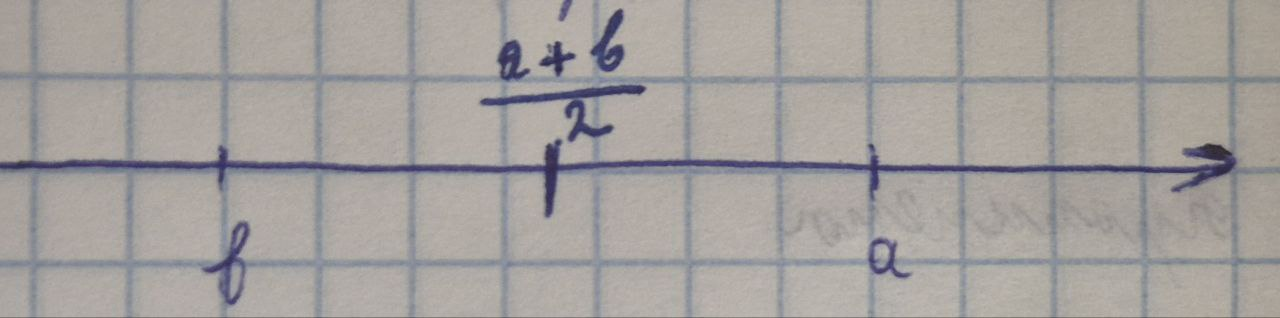
\includegraphics[width=0.5\linewidth]{III/Предельный переход}
	\end{center}
	\[ \exists n_\eps` \;\;\forall n > n_\eps` \;\; |a_n - a| < \eps \Leftrightarrow -\eps < a_n - a < \eps \Leftrightarrow a - \eps < a_n < a + \eps \]
	\[ \exists n_\eps`` \;\;\forall n > n_\eps`` \;\; |b_n - b| < \eps \Leftrightarrow -\eps < b_n - b < \eps \Leftrightarrow b - \eps < b_n < b + \eps \]
	\[ n_\eps = \max\{ n_\eps`, n_\eps``, N \} \]
	\[ \forall n > n_\eps: b_n < b + \eps = \frac{a + b}{2} = a-\eps < a_n \Rightarrow b_n < a_n ?! \]
\end{tcolorbox}
